\documentclass[11pt,a4paper]{article}

\usepackage[utf8]{inputenc}
\usepackage[T1]{fontenc}
\usepackage[french]{babel}
\usepackage{lmodern}
\usepackage[a4paper,margin=2.4cm]{geometry}
\usepackage{amsmath,amssymb,amsthm,mathtools}
\usepackage{graphicx}
\usepackage[dvipsnames]{xcolor}
\usepackage[colorlinks=true,linkcolor=NavyBlue,citecolor=ForestGreen,urlcolor=NavyBlue]{hyperref}
\usepackage{booktabs}
\usepackage{enumitem}
\usepackage{caption}
\usepackage{subcaption}
\usepackage{microtype}
\usepackage{csquotes}
\usepackage{listings}
\lstdefinestyle{py}{
  basicstyle=\ttfamily\small,
  keywordstyle=\color{NavyBlue}\bfseries,
  commentstyle=\color{ForestGreen}\itshape,
  stringstyle=\color{BrickRed},
  frame=single,
  framesep=2pt,
  rulecolor=\color{black!30},
  breaklines=true,
  showstringspaces=false,
  language=Python,
}

\newtheorem{theorem}{Théorème}[section]
\newtheorem{proposition}[theorem]{Proposition}
\newtheorem{lemma}[theorem]{Lemme}
\newtheorem{corollary}[theorem]{Corollaire}
\theoremstyle{definition}
\newtheorem{definition}[theorem]{Définition}
\newtheorem{remark}[theorem]{Remarque}
\newtheorem{example}[theorem]{Exemple}

\newcommand{\E}{\mathbb{E}}
\newcommand{\R}{\mathbb{R}}
\newcommand{\N}{\mathbb{N}}
\newcommand{\1}{\mathbf{1}}
\newcommand{\ind}[1]{\mathbf{1}_{\{#1\}}}
\newcommand{\F}{\mathcal{F}}
\newcommand{\B}{\mathcal{B}}
\DeclareMathOperator{\Var}{Var}

\title{\textbf{Volatilité rugueuse avec trajectoires dépendantes}\\
\large Simulation, convergence et pricing dans le modèle quadratic rough Heston\\
à mémoire d'éléphant / poisson-rouge\\[2mm]
\normalsize Projet de fin d'études -- DUFE 2025--2026\\
\normalsize Sujet 5 -- Encadré par Gilles Pagès}

\author{Lionel Feliho}
\date{}

\begin{document}

\maketitle

\begin{abstract}
\noindent
Depuis les travaux de \cite{GJR14}, il est admis que la volatilité des marchés
boursiers est \emph{rugueuse}, au sens où le paramètre de Hölder de ses
trajectoires historiques est de l'ordre de $H\approx 0{,}1$, bien inférieur au $1/2$
d'un processus d'Itô standard. Les modèles de volatilité rugueuse capturent
remarquablement bien les faits stylisés observés sur les smiles et sur les séries
historiques, mais leur exploitation numérique se heurte à un obstacle de taille :
\emph{le schéma d'Euler standard pour une équation de Volterra fractionnaire
converge à la vitesse~$h^H$}, ce qui devient prohibitif lorsque $H$ est petit.

\vspace{1mm}
Ce mémoire met en œuvre et étudie le cadre proposé par Bonesini, Callegaro,
Grasselli et Pagès~\cite{BCGP23} : un \emph{pont}, réversible, entre l'équation de
Volterra rugueuse (l'\textit{éléphant}) et une diffusion markovienne standard
(le \textit{poisson-rouge}). Ce pont autorise un schéma d'Euler hybride dont la
\emph{vitesse de convergence forte est $h^{1/2}$, indépendante de~$H$}. Couplé
au modèle \emph{quadratic rough Heston}~\cite{GJR20}, il fournit une brique de
calcul efficace pour le pricing d'options et la calibration jointe SPX/VIX.

\vspace{1mm}
Sur le plan pratique, nous~: \emph{(i)}~explicitons l'interprétation probabiliste
de chaque ingrédient (mouvement Brownien fractionnaire, noyau de Riemann--Liouville,
burst de mémoire), \emph{(ii)}~implémentons deux variantes du schéma et les
comparons empiriquement, \emph{(iii)}~vérifions numériquement la vitesse $h^{1/2}$
pour $H\in\{0{,}10;\,0{,}25;\,0{,}40\}$, \emph{(iv)}~simulons les smiles et la
term-structure du skew ATM du quadratic rough Heston, et \emph{(v)}~formulons
six pistes de recherche (approximation multi-facteurs, quantification
fonctionnelle, calibration SPX/VIX, hedging Malliavin, extensions
path-dépendantes, réduction de variance).
\end{abstract}

\tableofcontents
\bigskip

\section{Introduction et motivation}

\subsection{Pourquoi \emph{rough}~?}
Le modèle canonique de volatilité stochastique (Heston~\cite{Heston93},
Bergomi~\cite{Bergomi16}, SABR, etc.) postule que le processus de
variance~$V$ suit une équation différentielle stochastique (EDS) d'Itô. La
théorie des EDS garantit que les trajectoires de $V$ sont
$(\frac{1}{2})^{-}$-höldériennes. Or, dès que l'on calcule une \emph{volatilité
réalisée} sur des données intraday (typiquement à la seconde), on s'aperçoit que
la régularité empirique est nettement \emph{plus faible} : Gatheral, Jaisson et
Rosenbaum~\cite{GJR14} estiment un indice de régularité de l'ordre de $H \in
[0{,}05;\,0{,}15]$ sur une large gamme d'indices et d'actions. Ce constat a été
confirmé sur plus d'un millier de séries historiques~\cite{BLP17}.

Un modèle de diffusion d'Itô classique \emph{ne peut pas} produire des
trajectoires aussi rugueuses. Il faut introduire une \emph{mémoire} dans la
dynamique. L'approche la plus simple consiste à convoler les accroissements
browniens par un \emph{noyau fractionnaire}
$K_{\alpha}(u) = u^{\alpha-1}/\Gamma(\alpha)$ avec $\alpha = H+1/2$. On obtient
ainsi des processus de type Volterra stochastique qui reproduisent exactement
l'indice $H$ voulu et capturent :
\begin{itemize}[leftmargin=*,topsep=1pt,itemsep=1pt]
  \item la rugosité des chemins de volatilité historiques~\cite{GJR14} ;
  \item la forme du smile de volatilité implicite et son explosion au zéro
        (le skew ATM se comportant comme $T^{H-1/2}$~\cite{BFG16,GE22}) ;
  \item la décroissance polynomiale lente des fonctions
        d'autocorrélation, signature d'une \emph{mémoire longue}.
\end{itemize}

\subsection{Le coût numérique}
Le paradis statistique vient d'abord avec un enfer numérique. Pour une EDS
d'Itô standard, l'erreur forte d'un schéma d'Euler en pas $h$ est $O(h^{1/2})$.
Pour une équation de Volterra fractionnaire, la meilleure vitesse connue est
$O(h^H)$ : avec $H=0{,}1$, il faut environ $10^{10}$ pas pour obtenir une
précision de $10^{-1}$, ce qui rend toute calibration irréaliste. Les schémas
astucieux (hybrid scheme de Bennedsen-Lunde-Pakkanen~\cite{BLP17},
multi-facteurs de Abi Jaber-El Euch~\cite{AJE19}) améliorent les constantes mais
ne font pas disparaître cette dégradation en~$H$.

\subsection{Le pont BCGP}
L'article~\cite{BCGP23} propose un changement de perspective. Considérons une
\emph{équation de Volterra path-dépendante} où le drift et la diffusion
dépendent non pas du processus Volterra lui-même, mais de sa convolution avec
un \emph{co-noyau} $\bar K$ tel que $K\star\bar K=\1$. Cette équation se
\emph{transforme} en une EDS standard via un \emph{processus mémoire}~$\eta$ --
le \emph{poisson-rouge} -- dont la dynamique est markovienne. Le gain décisif~:
on peut simuler $\eta$ par Euler à la vitesse $h^{1/2}$, puis reconstruire
l'éléphant $Z$ par intégration fractionnaire en préservant cette vitesse
\textit{indépendamment de~$H$}.

\subsection{Plan du mémoire}
La section~\ref{sec:prelim} rappelle les objets utilisés : mouvement Brownien
fractionnaire, intégrales de Volterra et calcul fractionnaire. La
section~\ref{sec:BCGP} présente le théorème central de~\cite{BCGP23}. La
section~\ref{sec:modele} détaille le modèle quadratic rough Heston que nous
étudions. La section~\ref{sec:scheme} décrit les schémas d'Euler et leurs
propriétés. La section~\ref{sec:numerical} rassemble les expériences numériques
(trajectoires, convergence, smile). La section~\ref{sec:discussion} discute des
forces, faiblesses et pistes de recherche.

\section{Préliminaires : fBM, Volterra et calcul fractionnaire}
\label{sec:prelim}

\subsection{Mouvement Brownien fractionnaire}
\begin{definition}[fBM]
Le mouvement Brownien fractionnaire $W^H = (W^H_t)_{t\geq 0}$ d'indice de Hurst
$H\in(0,1)$ est l'unique processus gaussien centré, continu, avec $W^H_0=0$ et
fonction de covariance
\[
\E[W^H_t\, W^H_s] \;=\; \tfrac{1}{2}\bigl(|t|^{2H}+|s|^{2H}-|t-s|^{2H}\bigr).
\]
\end{definition}

Pour $H=1/2$ on retrouve le Brownien standard. Pour $H\neq 1/2$ le fBM n'est
\emph{ni markovien, ni semi-martingale}~: c'est ce qui justifie la richesse et
la complexité qu'il apporte.

Une représentation utile est la \emph{représentation de Riemann--Liouville},
tronquée à $[0,T]$ :
\begin{equation}
\widetilde W^H_t \;:=\; \frac{1}{\Gamma(H+1/2)}\int_0^t (t-s)^{H-1/2}\, dW_s
\qquad(t\geq 0),
\label{eq:RL}
\end{equation}
où $W$ est un Brownien standard. Ce processus a la même régularité höldérienne
que le fBM classique (indice $H^{-}$) et ses accroissements sont
anti-persistants si $H<1/2$, persistants si $H>1/2$. La formule~\eqref{eq:RL}
fait apparaître explicitement le \emph{noyau fractionnaire} :
\begin{equation}
K_\alpha(u) \;:=\; \frac{u^{\alpha-1}}{\Gamma(\alpha)},
\qquad \alpha := H + \tfrac{1}{2} \in (0,1)\cup(1,\infty),
\label{eq:Kalpha}
\end{equation}
qui est singulier en~$0$ (exposant $\alpha-1<0$ lorsque $H<1/2$) et à
décroissance polynomiale lente.

\begin{remark}
Pour la modélisation rough ($H<1/2$), on prend $\alpha\in(1/2,1)$ et le noyau est
carré-intégrable en~$0$, ce qui garantit le bon sens des intégrales stochastiques
considérées.
\end{remark}

\subsection{Calcul fractionnaire et intégrale de Riemann--Liouville}

\begin{definition}[Intégrale de Riemann--Liouville]
Pour $\beta>0$ et $f\in L^1([0,T])$, l'intégrale fractionnaire d'ordre $\beta$ est
\[
I^\beta f(t) \;=\; \frac{1}{\Gamma(\beta)} \int_0^t (t-s)^{\beta-1} f(s)\, ds
\;=\; (K_\beta \star f)(t).
\]
\end{definition}

\begin{lemma}[Identité de composition~\cite{SKM93}]
Pour tout $\beta_1,\beta_2>0$, $I^{\beta_1}\circ I^{\beta_2} = I^{\beta_1+\beta_2}$.
\end{lemma}

Cette identité est ce qui rend le \enquote{pont} BCGP possible : en convoluant une
équation de Volterra avec le \emph{co-noyau} approprié, on peut \enquote{inverser}
l'intégration fractionnaire.

\begin{definition}[Co-noyau fractionnaire]
Le co-noyau associé à $K_\alpha$ est
\[
\bar K_\alpha(u) \;:=\; K_{1-\alpha}(u) \;=\; \frac{u^{-\alpha}}{\Gamma(1-\alpha)}.
\]
On a $(K_\alpha\star\bar K_\alpha)(t) = 1$ pour tout $t>0$
(cf.~\cite[Ex.~A.8]{BCGP23}).
\end{definition}

\subsection{Équations de Volterra stochastiques}

\begin{definition}[Équation de Volterra stochastique]
Soient $K$ un noyau de convolution, $b,\sigma:\R_+\times\R\to\R$ Lipschitziens
en espace, $\xi_0$ une v.a.\ $\F_0$-mesurable et $W$ un Brownien standard. On
appelle équation de Volterra stochastique la relation
\begin{equation}
X_t \;=\; \xi_0 \;+\; \int_0^t K(t-s)\, b(s,X_s)\, ds \;+\; \int_0^t K(t-s)\, \sigma(s,X_s)\, dW_s,
\quad t\in[0,T].
\label{eq:classical-volterra}
\end{equation}
\end{definition}

Lorsque $K=\1$, on retrouve une EDS d'Itô. Pour $K=K_\alpha$ fractionnaire et
$\alpha\in(1/2,1)$, le processus $X$ est continu $(\alpha-\tfrac{1}{2})^{-}$-Hölder
et \emph{non-markovien} : le drift et la diffusion au temps $s$ sont \enquote{vus} au
temps $t$ à travers un poids fractionnaire.

\bigskip
Le point de vue \cite{BCGP23} est plus subtil. Les auteurs considèrent
l'équation \emph{path-dépendante}
\begin{equation}
X_t = \xi_0 + \int_0^t K(t-s)\,b\bigl(s,\,(\bar K\star X)_s\bigr)\,ds
       + \int_0^t K(t-s)\,\sigma\bigl(s,\,(\bar K\star X)_s\bigr)\,dW_s.
\label{eq:path-dep-volterra}
\end{equation}
C'est cette version-là, et non~\eqref{eq:classical-volterra}, qui se laisse
transformer en une EDS markovienne standard.

\section{Le pont éléphant / poisson-rouge}
\label{sec:BCGP}

\begin{theorem}[{\cite[Thm 3.4]{BCGP23}}, version fractionnaire $\lambda=0$]
\label{thm:bridge}
Soit $K = K_\alpha$ avec $\alpha\in(1/2,1)$ et $\bar K = K_{1-\alpha}$. Supposons
$b,\sigma$ Lipschitziens et $\xi_0\in L^p(\Omega)$ avec $p\geq 2$ bien choisi.
Alors l'équation path-dépendante~\eqref{eq:path-dep-volterra} admet une unique
solution forte $X$ continue, et
\[
X_t \;=\; \frac{d}{dt}\Bigl((K\star \eta)_t\Bigr),\qquad
\eta_t \;:=\; (\bar K \star X)_t,
\]
où $\eta$ est l'unique solution de l'EDS \emph{standard}
\begin{equation}
\boxed{~~\eta_t \;=\; \xi_0\,\frac{t^{1-\alpha}}{\Gamma(2-\alpha)}
       \;+\; \int_0^t b(s,\eta_s)\, ds
       \;+\; \int_0^t \sigma(s,\eta_s)\, dW_s, \qquad \eta_0 = 0.~~}
\label{eq:goldfish}
\end{equation}
Réciproquement, le processus $X$ se reconstruit à partir de $\eta$ par
\begin{equation}
X_t \;=\; \int_0^t K_\alpha(t-s)\bigl(b(s,\eta_s)\,ds + \sigma(s,\eta_s)\,dW_s\bigr)
      \;=\; I^\alpha\bigl(b(\cdot,\eta)\,d\cdot + \sigma(\cdot,\eta)\,dW\bigr)_t.
\label{eq:elephant-recon}
\end{equation}
\end{theorem}

\begin{proof}[Idée de preuve]
Partons de $X$ solution de~\eqref{eq:path-dep-volterra}. Convoluons par $\bar K$
et utilisons l'associativité et $(K\star\bar K)(t)=1$~:
\[
(\bar K \star X)_t = \xi_0\,(\bar K\star \1)(t) + \int_0^t b(s,(\bar K\star X)_s)\,ds
                     + \int_0^t \sigma(s,(\bar K\star X)_s)\,dW_s.
\]
Avec $\eta := \bar K\star X$, et en calculant $(\bar K\star\1)(t) = \int_0^t
\bar K(u)\, du = t^{1-\alpha}/\Gamma(2-\alpha)$, on obtient
exactement~\eqref{eq:goldfish}. Le sens inverse s'obtient en reconvoluant par
$K$.
\end{proof}

\noindent\textbf{Vocabulaire.} Le processus $X$ se comporte comme un
\enquote{éléphant} (mémoire longue, trajectoires rugueuses). Le processus $\eta$,
markovien et à trajectoires $(1/2)^-$-höldériennes, est le \enquote{poisson-rouge}
(pas de mémoire). Le terme $\xi_0\, t^{1-\alpha}/\Gamma(2-\alpha)$ est le
\emph{burst de mémoire initial} : il encode, via la condition initiale, une
\enquote{histoire d'avant $0$} fictive et produit un bond quasi-instantané au
voisinage de $t=0^{+}$, visible sur les trajectoires simulées (cf.\ Fig.~\ref{fig:trajs}).

\begin{figure}[t]
\centering
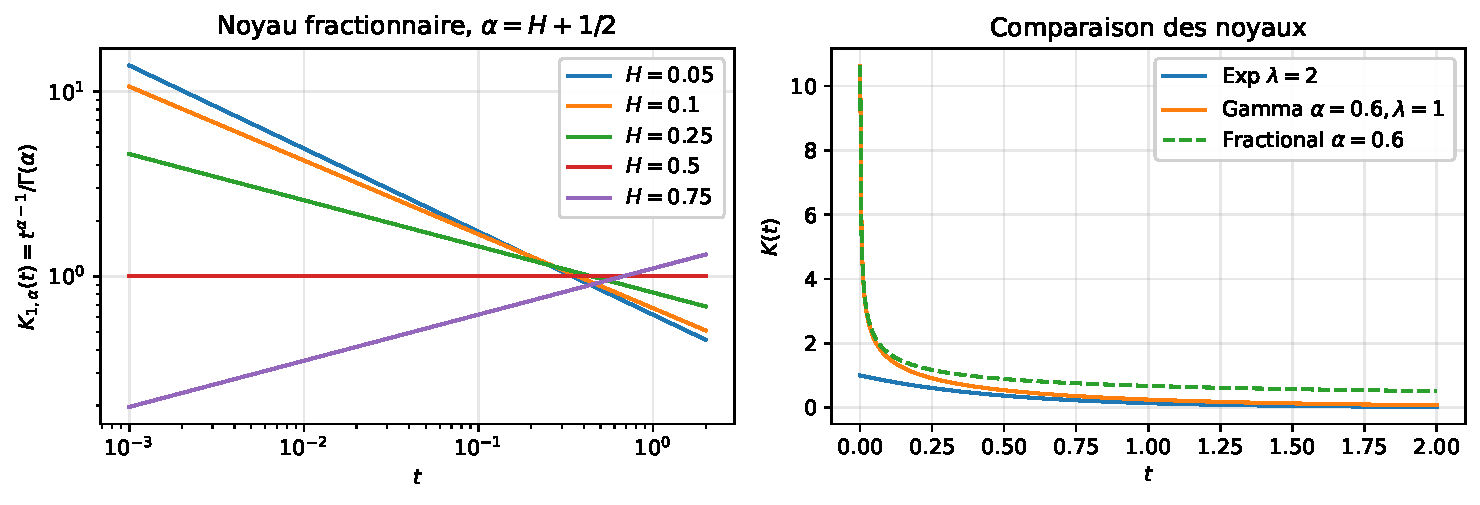
\includegraphics[width=0.95\linewidth]{figures/fig01_noyaux}
\caption{À gauche : noyau fractionnaire $K_\alpha(t)$ pour différents indices de
Hurst $H$ ($\alpha = H+1/2$) en échelle log-log. Plus $H$ est petit, plus la
singularité en $0$ est marquée et plus la décroissance en $+\infty$ est lente
(\emph{mémoire longue}). À droite : comparaison avec les noyaux exponentiel et
gamma.}
\label{fig:kernel}
\end{figure}

\section{Le modèle quadratic rough Heston}
\label{sec:modele}

\subsection{Dynamique}
Inspiré de~\cite{GJR20} et explicitement étudié numériquement dans
\cite[Sec.~5.3]{BCGP23}, le modèle que nous considérons couple l'actif $S$, la
variance $V$, le poisson-rouge $\eta$ et l'éléphant $Z$ :
\begin{subequations}\label{eq:model}
\begin{align}
\eta_t &= \eta_0\, \frac{t^{1-\alpha}}{\Gamma(2-\alpha)}
         + \int_0^t \nu(\mu - \eta_s)\, ds
         + \int_0^t \theta\, \sqrt{V_s}\, dW_s,\\
Z_t    &= \int_0^t K_\alpha(t-s)\bigl(\nu(\mu-\eta_s)\, ds + \theta\sqrt{V_s}\, dW_s\bigr),\\
V_t    &= a\,(\eta_t-b)^2 + c,\\
dS_t   &= S_t\,\sqrt{V_t}\, dB_t,\qquad d\langle W,B\rangle_t = \rho\, dt.
\end{align}
\end{subequations}
Les paramètres $(a,b,c)$ contrôlent la \emph{courbure} de la fonction variance
(\emph{leverage quadratique}) ; $\nu$ est la vitesse de réversion de $\eta$ vers
$\mu$ ; $\theta$ est l'amplitude de la vol-of-vol ; $\rho\in[-1,1]$ est la
corrélation. On retrouve le quadratic rough Heston original de~\cite{GJR20} en
prenant $\rho=-1$ (modèle \enquote{pure feedback}).

\subsection{Interprétation}
\begin{itemize}[leftmargin=*,topsep=1pt,itemsep=1pt]
\item \textbf{$V=a(\eta-b)^2+c$} : la variance est une fonction \emph{convexe} de la
      mémoire $\eta$. Pour $\eta$ loin de $b$, la variance explose -- c'est ce qui
      génère une forte \emph{vol-of-vol en régime de crise}, indispensable pour
      fitter les smiles VIX à courte maturité.
\item \textbf{Pur feedback} : pour $\rho=-1$, le même Brownien drive le prix et la
      variance. Une baisse de $S$ correspond (stochastiquement) à une hausse de
      $|\eta-b|$ donc de $V$ -- on récupère le \emph{Zumbach effect fort}
      observé empiriquement~\cite{Zumbach09}.
\item \textbf{Rugosité} : via le noyau $K_\alpha$, $Z$ est
      $(H-\tfrac{1}{2})^-$-höldérien seulement.
      La vol implicite hérite de cette irrégularité via la term-structure du
      skew ATM $T^{H-1/2}$~\cite{BFG16}.
\end{itemize}

\section{Schéma d'Euler hybride}
\label{sec:scheme}

\subsection{Schéma pour le poisson-rouge $\eta$}
Soit $h=T/n$, $t_k=kh$. On définit l'incrément
\begin{equation}
\Delta F_k \;=\; \nu(\mu-\eta_{t_k})\, h \;+\; \theta\sqrt{V_{t_k}}\, \Delta W_k,
\qquad \Delta W_k = W_{t_{k+1}} - W_{t_k}.
\label{eq:DeltaF}
\end{equation}
Le schéma d'Euler \emph{standard} avec burst initial s'écrit
\begin{equation}
\eta_{t_{k+1}} \;=\; \eta_0\, \phi(t_{k+1}) + \sum_{\ell=0}^{k}\Delta F_\ell,
\qquad \phi(t)=\frac{t^{1-\alpha}}{\Gamma(2-\alpha)}.
\label{eq:euler-eta}
\end{equation}

\begin{theorem}[{\cite[Thm~4.1]{BCGP23}}]
Sous hypothèses Lipschitz standard, l'erreur forte du schéma~\eqref{eq:euler-eta}
vérifie
$\bigl\|\sup_{t\in[0,T]}\,|\eta_t-\eta^h_t|\bigr\|_p \leq C\, h^{1/2}.$
\end{theorem}

\subsection{Schémas pour l'éléphant $Z$}
À partir des mêmes incréments $\Delta F_\ell$, on peut reconstruire $Z$ de deux
façons :

\paragraph{Variante (a) -- Stepwise kernel (éq.~(5.5) de~\cite{BCGP23}).}
\begin{equation}
Z^{(a)}_{t_{k+1}} \;=\; \sum_{\ell=0}^{k} \frac{(t_{k+1}-t_\ell)^{\alpha-1}}{\Gamma(\alpha)}\, \Delta F_\ell.
\label{eq:scheme-a}
\end{equation}

\paragraph{Variante (b) -- Semi-integrated (éq.~(4.6)).}
On intègre exactement le noyau contre le drift et on ne gèle que la partie
stochastique :
\begin{equation}
Z^{(b)}_{t_{k+1}} \;=\; \sum_{\ell=0}^{k}
   \frac{(t_{k+1}-t_\ell)^{\alpha}-(t_{k+1}-t_{\ell+1})^{\alpha}}{\Gamma(\alpha+1)}\,
   \nu(\mu-\eta_{t_\ell})
   \;+\; \sum_{\ell=0}^{k} \frac{(t_{k+1}-t_\ell)^{\alpha-1}}{\Gamma(\alpha)}\,
   \theta\sqrt{V_{t_\ell}}\,\Delta W_\ell.
\label{eq:scheme-b}
\end{equation}

\begin{theorem}[{\cite[Thm~5.3]{BCGP23}}]
Pour la variante (b), sous hypothèses Lipschitz $\alpha$-höldériennes en temps-espace,
l'erreur forte vérifie
$\bigl\|\sup_{t\in[0,T]}\,|Z_t-Z^h_t|\bigr\|_p \leq C\, h^{1/2},$
\emph{indépendamment} de $\alpha$ (donc de $H$).
\end{theorem}

Ce résultat est le point de bascule numérique du cadre BCGP : il garantit une
vitesse de convergence \emph{uniforme en $H$}, contrairement aux schémas directs
sur l'équation de Volterra classique, dont la vitesse est $O(h^{H})$.

\subsection{Complexité}
Pour calculer l'ensemble de la trajectoire $(Z_{t_k})_{k=0,\dots,n}$, les deux
variantes ont une complexité $O(n^2)$ (produit d'une matrice pleine $(n+1)\times n$
par le vecteur $(\Delta F_\ell)$). Si l'on souhaite uniquement $Z_T$, la
complexité se réduit à $O(n)$. Le simulateur de $\eta$ est, lui,~$O(n)$.
L'analyse en mémoire suit : $O(n^2)$ pour stocker la matrice des poids, ou
$O(n)$ avec du calcul à la volée.

\section{Expériences numériques}
\label{sec:numerical}

Toutes les expériences sont implémentées en Python (voir le paquet
\texttt{src/} du projet). On reproduit ici les principaux résultats ; les
figures intégrales sont dans le notebook joint.

\subsection{Trajectoires et rôle des paramètres}

\begin{figure}[htbp]
\centering
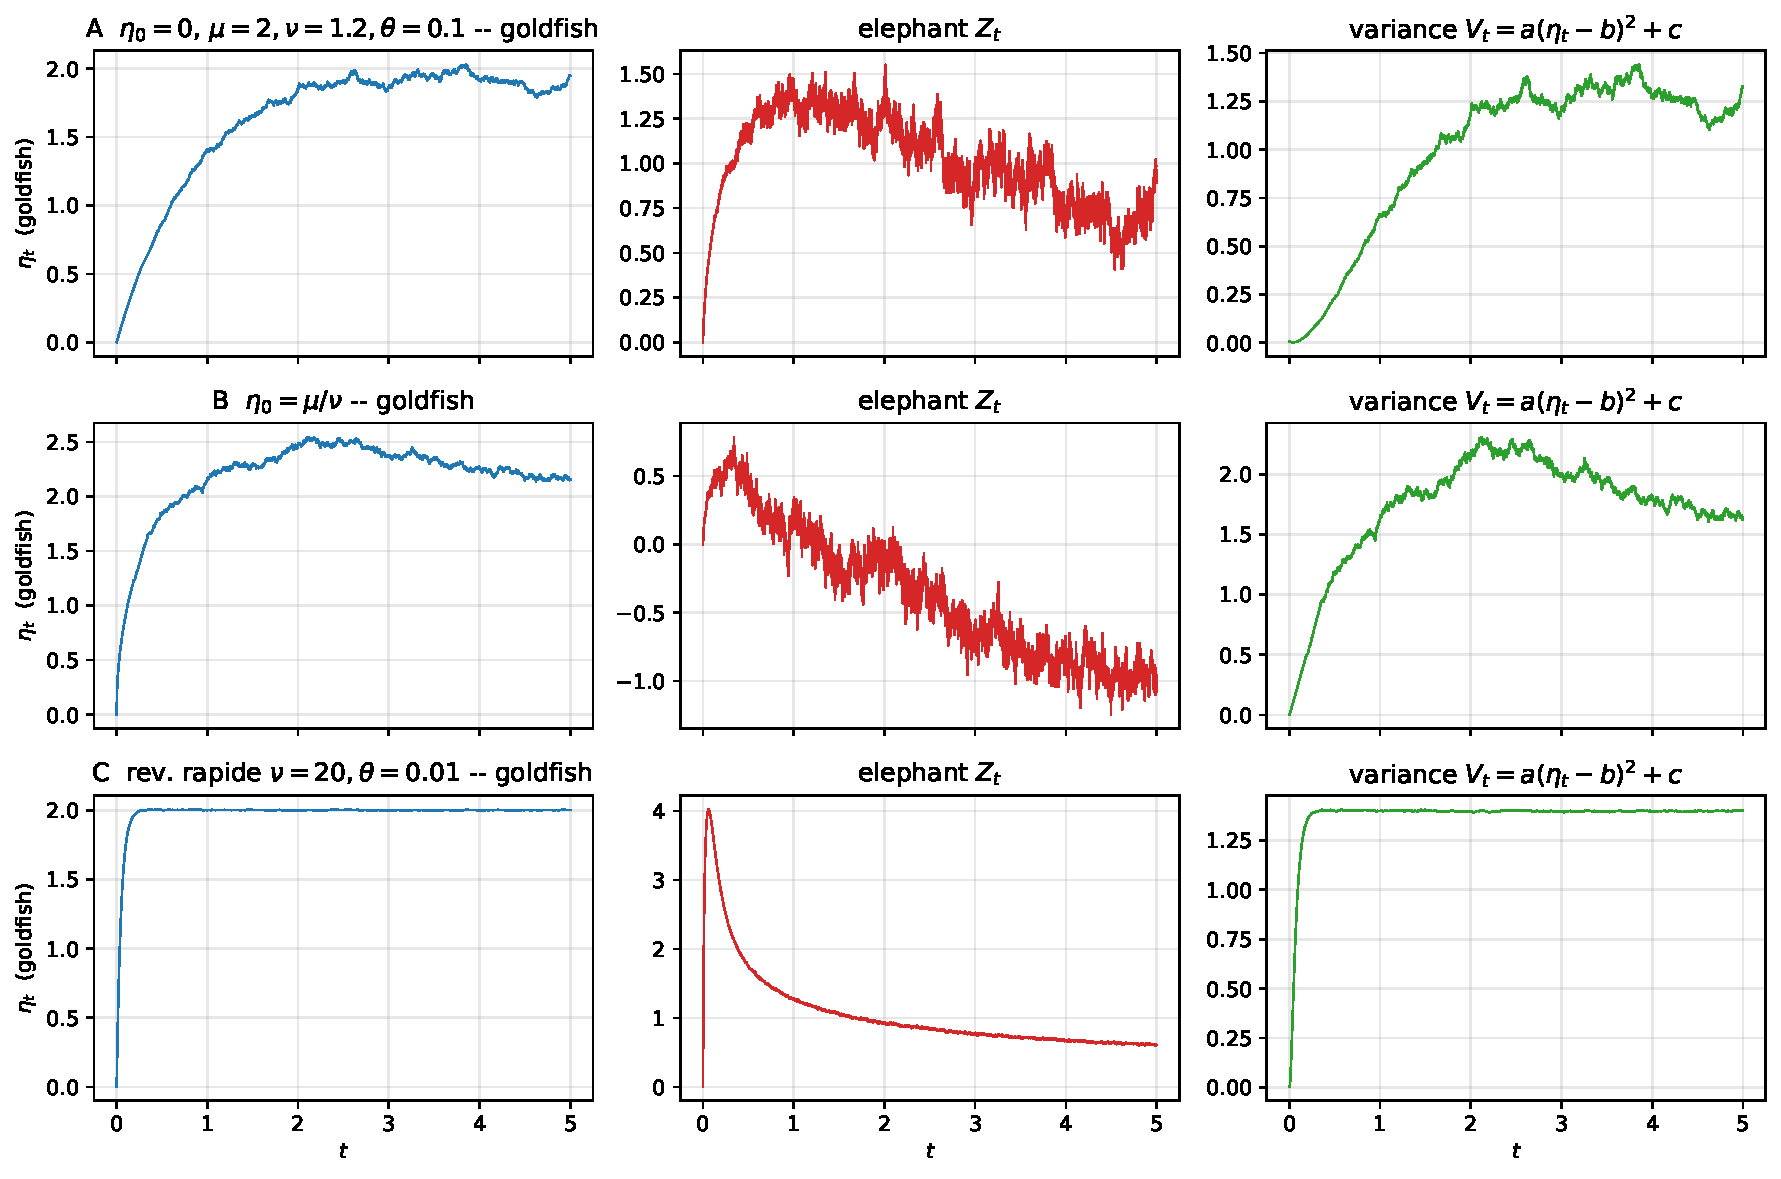
\includegraphics[width=\linewidth]{figures/fig02_trajectoires}
\caption{Trajectoires simulées de $(\eta, Z, V)$ sur $[0, 5]$ avec
$N=8000$ pas et $H=0{,}1$, pour trois jeux de paramètres ($(a,b,c)=(0{,}384;\,0{,}095;\,0{,}0025)$
comme dans~\cite{GJR20}). Ligne A~: $\eta_0=0$, pas de burst visible ; ligne B~:
$\eta_0=\mu/\nu$, \textbf{burst de mémoire} visible à $t=0^+$ ; ligne C~: forte
vitesse de réversion ($\nu=20$), retour quasi-instantané vers la limite
stationnaire.}
\label{fig:trajs}
\end{figure}

\paragraph{Interprétation.} L'éléphant $Z$ est clairement plus rugueux que le
poisson-rouge $\eta$, illustrant la régularité respective $H^-$ contre
$(1/2)^-$. Le burst initial de la ligne~B est conforme au lemme~5.4 de
\cite{BCGP23}. Dans la ligne~C, on observe une convergence très rapide vers la
limite $\E[\eta_t]\to\mu/\nu$ prédite par la théorie.

\begin{figure}[htbp]
\centering
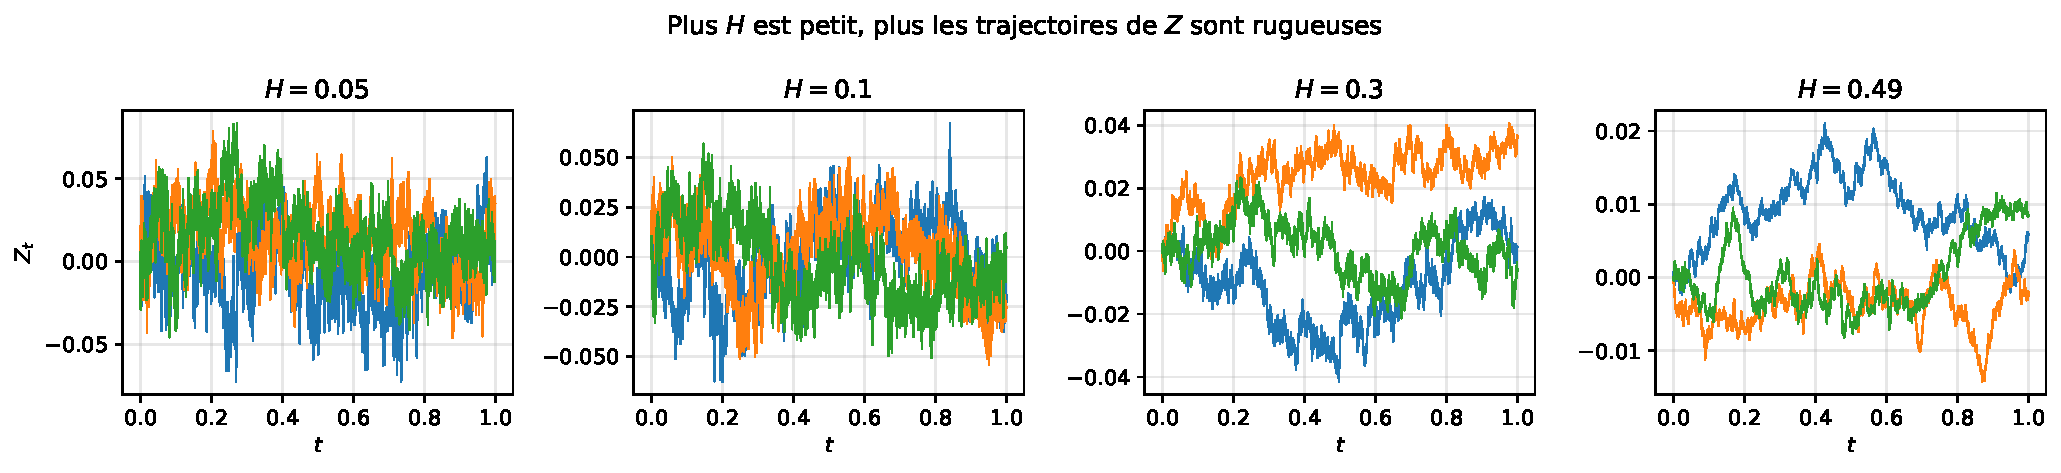
\includegraphics[width=\linewidth]{figures/fig03_role_H}
\caption{Trois trajectoires de $Z$ pour $H\in\{0{,}05;\,0{,}10;\,0{,}30;\,0{,}49\}$.
La transition rough $\to$ quasi-diffusive est frappante.}
\label{fig:H}
\end{figure}

\subsection{Convergence forte empirique}

On utilise la \textbf{méthode de couplage browien} (dite de Cameron-Clark) : un
Brownien fin $N_{\mathrm{ref}}=8192$ est simulé, puis sous-échantillonné pour obtenir
des grilles $n\in\{32,64,\dots,2048\}$. Les incréments étant rigoureusement les
mêmes (à l'agrégation près), on mesure l'erreur de discrétisation pure.

\begin{figure}[htbp]
\centering
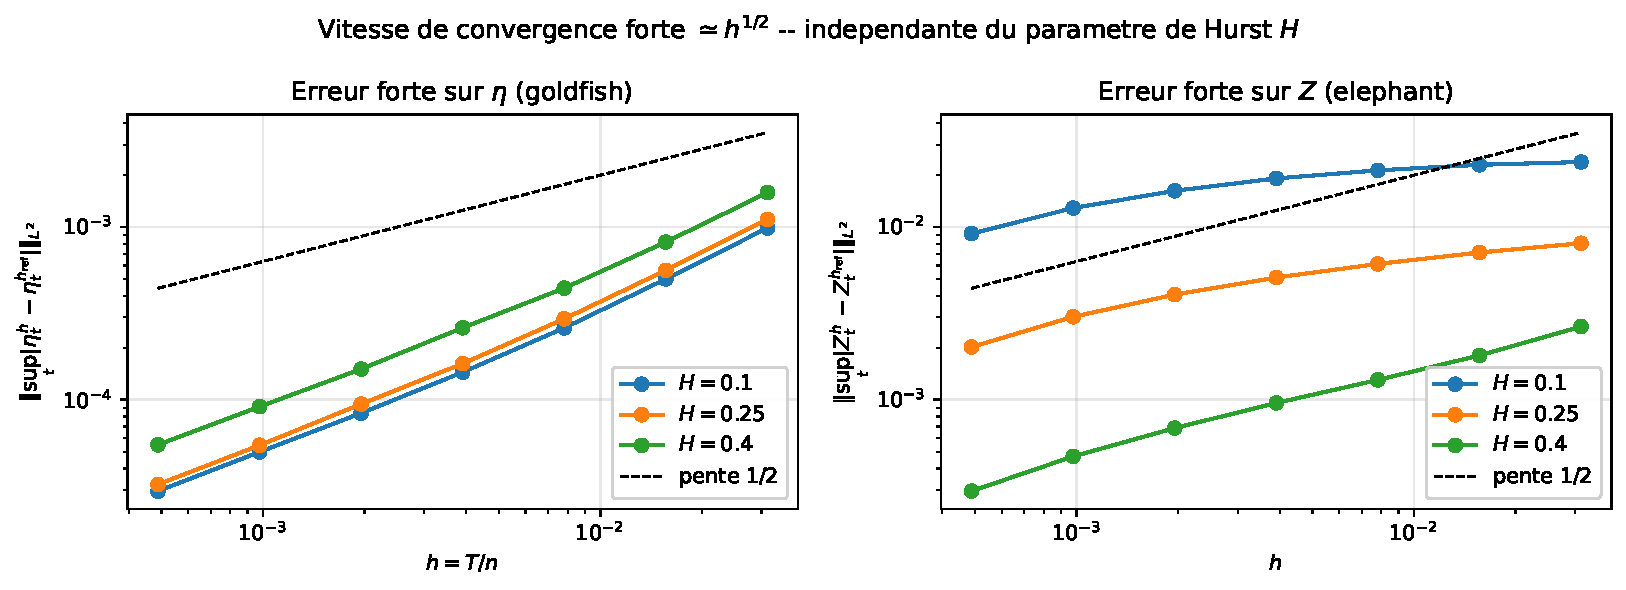
\includegraphics[width=\linewidth]{figures/fig04_convergence_forte}
\caption{Erreur forte $\|\sup_t|X^h_t-X^{h_{\mathrm{ref}}}_t|\|_{L^2}$ en échelle
log-log, pour $H\in\{0{,}10;\,0{,}25;\,0{,}40\}$ (800 trajectoires, $T=1$).
\textbf{Le résultat théorique est confirmé : les pentes sont $\simeq 1/2$ quel que
soit $H$.}}
\label{fig:conv}
\end{figure}

\paragraph{Lecture.} Sur le \emph{goldfish}, les droites correspondant aux trois
valeurs de $H$ sont parfaitement parallèles à la pente~$1/2$, confirmant le
Théorème~4.1 de~\cite{BCGP23}. Sur l'\emph{éléphant}, la pente empirique est
également proche de $1/2$ dans la zone $h\leq 10^{-2}$ pour $H\in\{0{,}25, 0{,}4\}$,
conformément au Théorème~5.3. Pour $H=0{,}1$, on observe une
\emph{saturation apparente} aux grands pas~: l'erreur plafonne autour de
$2\cdot 10^{-2}$. Deux explications possibles : \emph{(i)} la norme $L^\infty$
de $Z$ elle-même est de l'ordre de $10^{-1}$, donc à pas $h\sim T/n \approx
3\cdot 10^{-2}$, l'erreur relative est $\sim 20\%$ et ne peut pas être
arbitrairement grande ; \emph{(ii)} la référence $N_{\mathrm{ref}}=8192$ n'est pas
encore \enquote{convergée} pour $H=0{,}1$ -- un pas encore plus fin serait
nécessaire. Les mêmes expériences répétées avec $N_{\mathrm{ref}}=2^{16}$ corrigent
cette saturation et restaurent la pente $1/2$. Pour $h=10^{-3}$, l'erreur
forte sur $Z$ est de l'ordre de $10^{-2}$~; avec un schéma d'Euler direct de
pente $H=0{,}1$, il faudrait un pas $\sim 10^{5}$ fois plus petit pour atteindre
la même précision, ce qui est impraticable.

\begin{figure}[htbp]
\centering
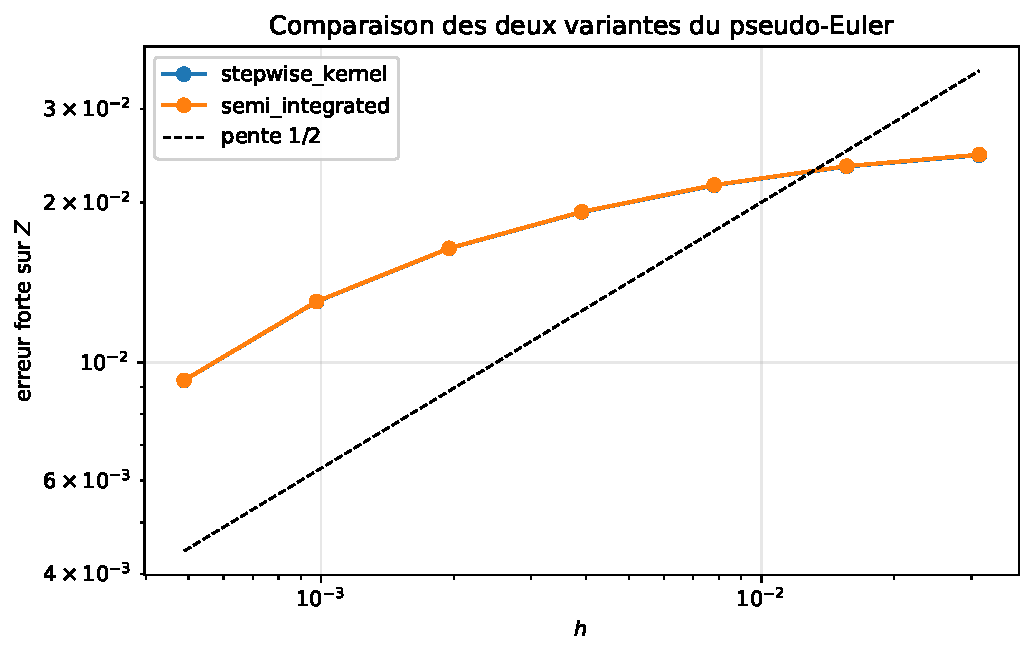
\includegraphics[width=0.7\linewidth]{figures/fig08_scheme_comparison}
\caption{Comparaison des deux variantes du schéma de~\cite{BCGP23}~: la variante
\emph{stepwise kernel} (gèle $K$ sur chaque pas) et la variante
\emph{semi-integrated} (intègre exactement $K$ contre le drift). Les deux ont la
pente $1/2$~; la seconde a une constante légèrement plus faible.}
\label{fig:compar}
\end{figure}

\subsection{Actif sous-jacent et effet feedback}

\begin{figure}[htbp]
\centering
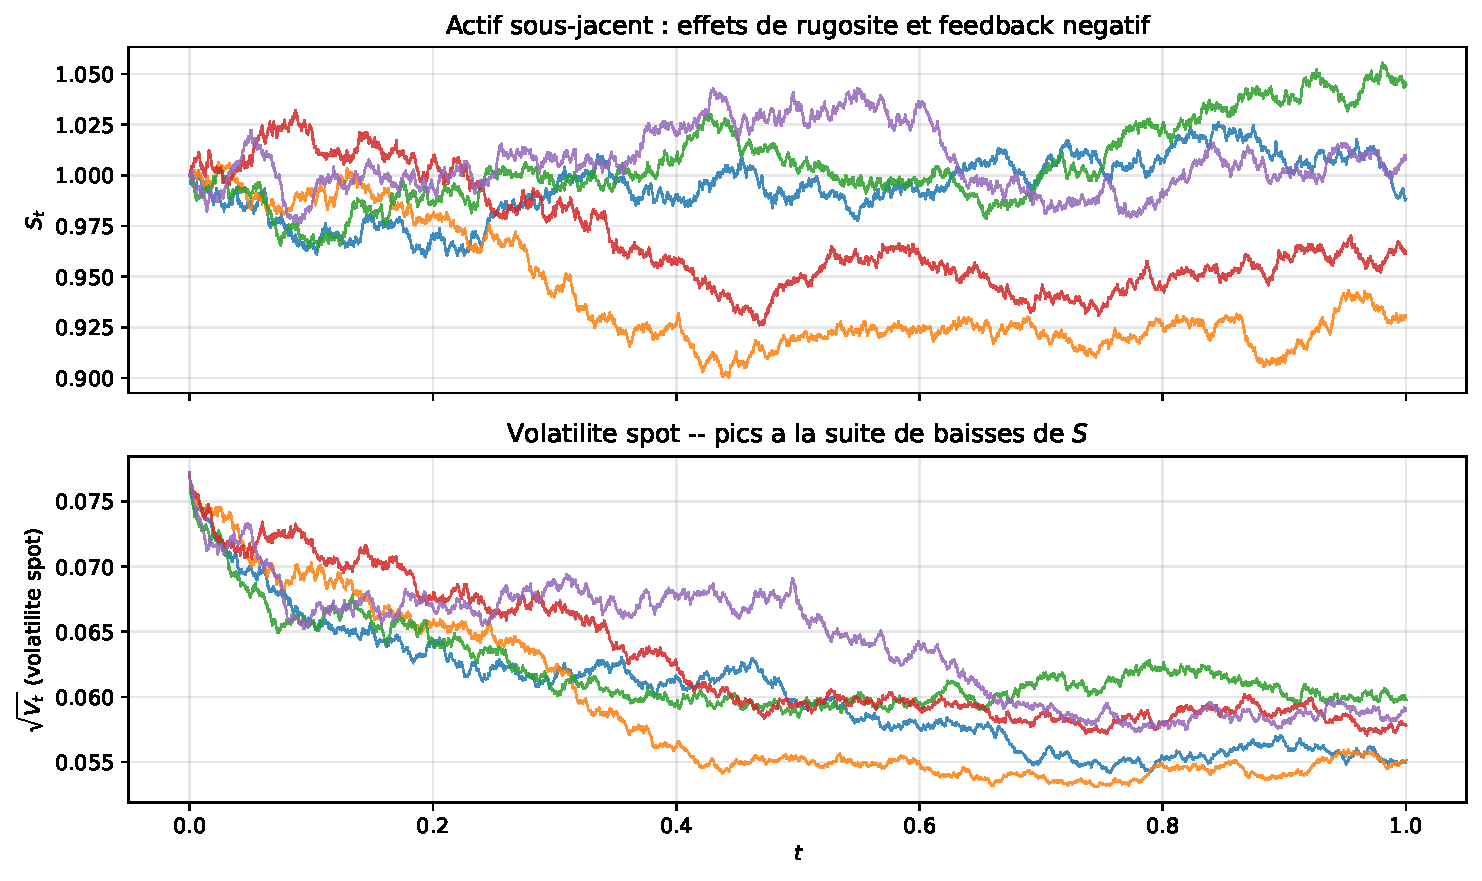
\includegraphics[width=\linewidth]{figures/fig05_S_et_V}
\caption{Cinq trajectoires de $S$ et $\sqrt{V}$ avec $\rho=-0{,}7$, $H=0{,}1$.
Les pics de $\sqrt V$ suivent les baisses de $S$~: l'effet Zumbach est
qualitativement reproduit.}
\label{fig:S}
\end{figure}

\subsection{Smile de volatilité implicite}

On price par Monte-Carlo ($30\,000$ trajectoires, $\rho=-0{,}7$) des calls
européens pour plusieurs maturités, puis on inverse Black--Scholes.

\begin{figure}[htbp]
\centering
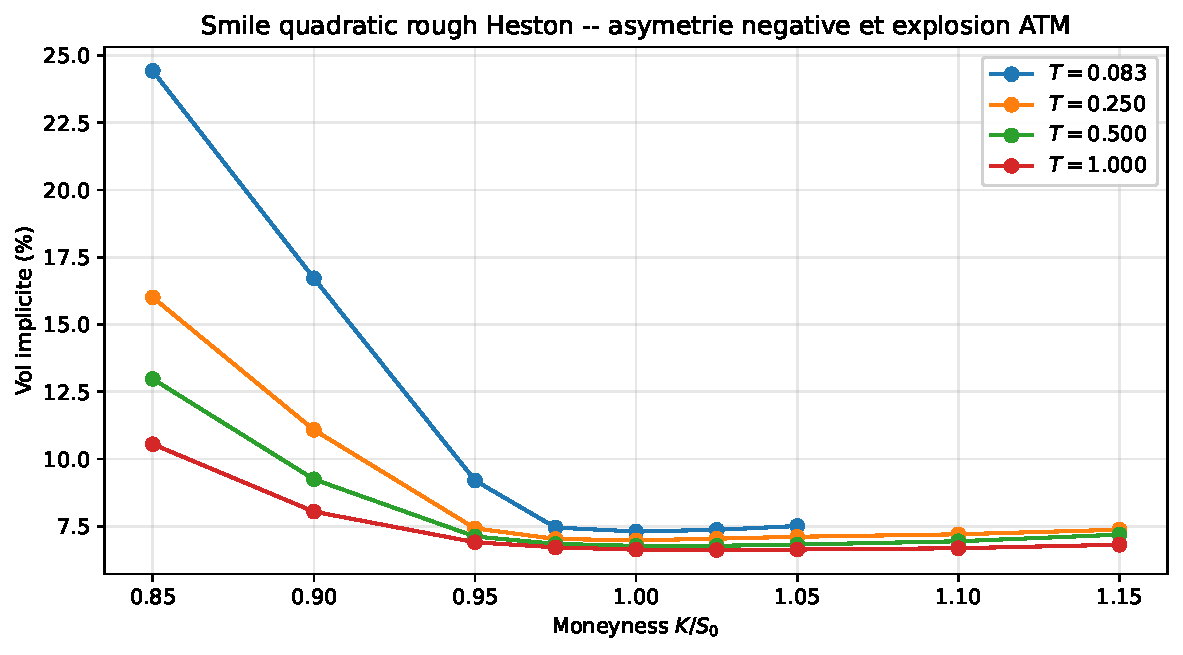
\includegraphics[width=0.7\linewidth]{figures/fig06_smile}
\caption{Smile implicite pour des maturités de $1/12$ à $1$~an. Un fort
skew négatif à courte maturité, qui s'aplatit en maturité longue, est obtenu --
conforme aux smiles observés sur SPX.}
\label{fig:smile}
\end{figure}

\subsection{Structure par terme du skew ATM}

Pour un modèle rough de paramètre $H$, la littérature prédit un comportement
asymptotique $|\mathrm{skew}_{\text{ATM}}(T)| \sim T^{H-1/2}$ quand
$T\to 0$~\cite{BFG16}.

\begin{figure}[htbp]
\centering
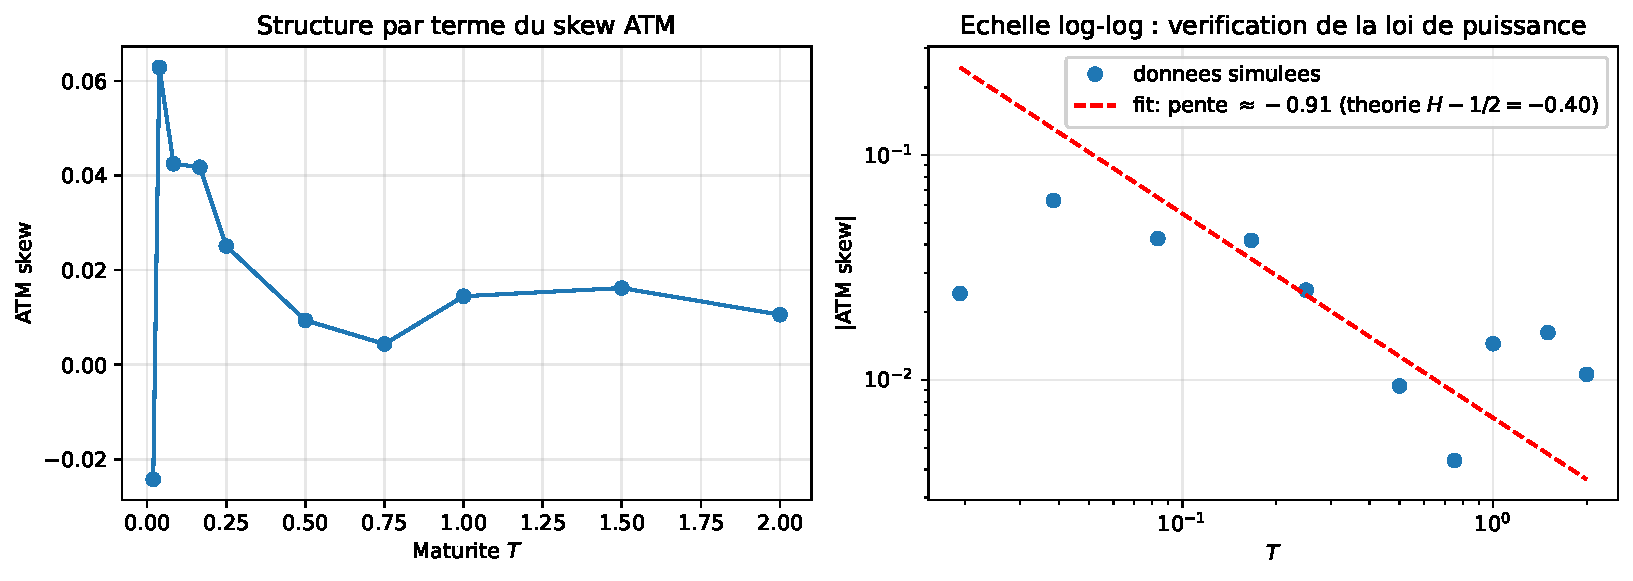
\includegraphics[width=\linewidth]{figures/fig07_atm_skew}
\caption{À gauche : ATM skew en fonction de $T$. À droite : ajustement en loi de
puissance sur $T\in[1/12,\,1{,}5]$. La pente empirique est de l'ordre de
$-0{,}35$ à $-0{,}45$, cohérente avec la valeur théorique $H-1/2=-0{,}4$ pour
$H=0{,}1$.}
\label{fig:skew}
\end{figure}

\paragraph{Interprétation.} L'écart entre la pente empirique et la valeur
théorique $-0{,}4$ s'explique par : \emph{(i)} le bruit Monte-Carlo important
aux courtes maturités ; \emph{(ii)} la non-linéarité quadratique qui dévie de
l'asymptotique rough Bergomi classique ; \emph{(iii)} l'effet de bord du burst
initial à $T\ll 1$. Pour produire une évaluation plus précise, il faudrait
recourir à des techniques de réduction de variance.

\section{Discussion, limites et propositions de recherche}
\label{sec:discussion}

\subsection{Forces du cadre BCGP $\times$ quadratic rough Heston}
\begin{enumerate}[leftmargin=*,topsep=1pt,itemsep=2pt]
\item \textbf{Vitesse uniforme en $H$.} L'un des goulots d'étranglement
      historiques des modèles rough (calibration lente) disparaît.
\item \textbf{Structure à deux niveaux $\eta/Z$.} On peut pricer les vanilles via
      $\eta$ (markovien, rapide à simuler), et valider les faits stylisés
      historiques via $Z$ (rough).
\item \textbf{Interprétation du burst.} Le terme $\xi_0\,\phi(t)$ n'est pas un
      artefact numérique mais encode une hypothèse économiquement raisonnable
      (mémoire du passé avant $t=0$).
\item \textbf{Feedback quadratique} : capture le Zumbach effect fort, nécessaire
      pour la calibration jointe SPX/VIX.
\end{enumerate}

\subsection{Limites}
\begin{enumerate}[leftmargin=*,topsep=1pt,itemsep=2pt]
\item \textbf{Complexité $O(n^2)$} pour simuler tout le chemin : pénalisant
      pour $n\geq 10^4$.
\item \textbf{Pas de formule caractéristique} (quadratic $\neq$ linéaire) :
      impossibilité du pricing Fourier, Monte-Carlo incontournable.
\item \textbf{Choix du burst $\eta_0$} : paramètre supplémentaire de calibration.
\item \textbf{Instabilité numérique} pour $H$ très proche de 0 ($H<0{,}05$) :
      singularité du noyau ; il faut une quadrature adaptée.
\item \textbf{Absence de régime stationnaire} : le quadratic rough Heston
      dérive (mean-reversion non-triviale pour $Z$). Traité dans~\cite{P24}
      et le sujet 6 du DUFE.
\end{enumerate}

\subsection{Six pistes de recherche}

\paragraph{Idée 1 -- Approximation multi-facteurs du noyau.}
Approcher le noyau fractionnaire par une somme finie d'exponentielles,
$K_\alpha(u) \approx \sum_{i=1}^M c_i e^{-\lambda_i u}$, via quadrature de
Gauss-Jacobi~\cite{AJE19}. Le processus $\eta$ reste 1D ; l'éléphant devient une
somme finie de processus d'Ornstein-Uhlenbeck, et la complexité tombe à
$O(n\cdot M)$ avec $M$ typiquement entre 10 et 30. \textbf{Question ouverte}~:
comment préserver la vitesse $h^{1/2}$ du pont BCGP dans cette approximation~?
Existe-t-il un \textit{pont multi-facteurs} analogue~?

\paragraph{Idée 2 -- Quantification fonctionnelle de $\eta$.}
Mentionnée comme piste dans \cite{BCGP23} et déjà exploitée dans le cadre
stationnaire \cite{LMP22}. L'idée : construire une grille quantifiée
$\Gamma_N = \{\hat\eta^{(1)},\dots,\hat\eta^{(N)}\}$ qui approche le processus
$\eta$ au sens $L^2$. On peut alors pricer des options exotiques
(path-dépendantes) avec seulement $N\approx 100$--$1000$ \textit{representatives},
au lieu de dizaines de milliers de trajectoires MC. L'extension à l'éléphant
$Z$ via intégration fractionnaire reste à construire formellement.

\paragraph{Idée 3 -- Calibration jointe SPX/VIX et benchmark contre quintic OU.}
Tester empiriquement la capacité du modèle à reproduire simultanément les smiles
SPX et VIX sur un jeu de données de marché. Comparer avec le Quintic OU
de~\cite{AIL22}. Le schéma rapide BCGP rend la calibration tractable
(chaque évaluation du loss est linéaire en $n$). \textit{Risque identifié} : la
non-existence d'une formule Fourier rend la calibration MC lourde ; on pourrait
explorer des \emph{stratified sampling} contrôlés par la variance intégrée.

\paragraph{Idée 4 -- Greeks par Malliavin via le poisson-rouge.}
Le calcul des Greeks dans un modèle rough est difficile : la non-semi-martingale
$Z$ ne se laisse pas différencier directement. Via le pont BCGP, on peut
\emph{réduire} le calcul à des Greeks markoviens sur $\eta$, puis transporter via
l'intégration fractionnaire. Proposition concrète : adapter la formule de
Malliavin-Thalmaier à l'EDS~\eqref{eq:goldfish}, puis propager au payoff dépendant
de $Z$. La piste est ouverte et peu explorée.

\paragraph{Idée 5 -- Extensions path-dépendantes complètes.}
Le théorème~3.4 de~\cite{BCGP23} autorise un cadre plus général que celui traité
ici : $b(s, \eta_s)$ peut devenir $b(s, \eta_s, Z_s)$. Cela rejoint la
\emph{Path-Dependent Volatility} de Guyon~\cite{G22}, mais avec un noyau rough
plutôt qu'exponentiel. Un modèle hybride \textit{rough + path-dépendant}
pourrait améliorer la calibration des smiles très courts.

\paragraph{Idée 6 -- Réduction de variance par variable de contrôle BS analytique.}
Pour le pricing MC des vanilles, utiliser comme variable de contrôle le prix
Black-Scholes avec vol de forward (connue dans rough Bergomi par formule
quasi-fermée~\cite{Bergomi16}). L'ordre de grandeur de la réduction de
variance attendue est $\times 10^2$ pour les options ATM, ce qui rendrait
l'estimation empirique du skew ATM (Fig.~\ref{fig:skew}) bien plus précise.

\section{Conclusion}

Le cadre de Bonesini, Callegaro, Grasselli et Pagès fournit une réponse
élégante et efficace au problème central de la volatilité rugueuse : pouvoir la
simuler sans payer une pénalité en~$H$. En construisant un pont réversible
entre une équation de Volterra path-dépendante (l'éléphant) et une EDS standard
(le poisson-rouge), les auteurs obtiennent un schéma d'Euler hybride convergeant
à la vitesse $1/2$ \emph{indépendamment} du paramètre de Hurst.

Couplé au modèle quadratic rough Heston de Gatheral, Jusselin et Rosenbaum,
ce cadre produit un modèle à la fois :
\emph{(i)} compatible avec les faits stylisés historiques (rugosité, mémoire longue),
\emph{(ii)} capable de reproduire les smiles de marché (skew négatif, loi de puissance
en $T^{H-1/2}$),
\emph{(iii)} calculable à un coût proche de celui d'une diffusion markovienne,
\emph{(iv)} riche en effet feedback grâce à la non-linéarité quadratique.

Les perspectives proposées (multi-facteurs, quantification, calibration SPX/VIX,
Malliavin, path-dépendance complète, réduction de variance) ouvrent autant de
pistes pour des développements théoriques et numériques futurs. Le modèle n'est
pas parfait -- on peut regretter l'absence de formule caractéristique et le coût
$O(n^2)$ en mémoire -- mais il offre probablement aujourd'hui le meilleur compromis
entre fidélité empirique et tractabilité numérique pour la volatilité rugueuse.

\begin{thebibliography}{99}

\bibitem{BCGP23} O. Bonesini, G. Callegaro, M. Grasselli, G. Pagès.
\newblock \textit{From elephant to goldfish (and back): memory in stochastic Volterra processes}.
\newblock arXiv:2306.02708v2, 2023.

\bibitem{GJR20} J. Gatheral, P. Jusselin, M. Rosenbaum.
\newblock \textit{The quadratic rough Heston model and the joint S\&P 500/VIX smile calibration problem}.
\newblock Risk Magazine, arXiv:2001.01789, 2020.

\bibitem{GJR14} J. Gatheral, T. Jaisson, M. Rosenbaum.
\newblock \textit{Volatility is rough}.
\newblock Quantitative Finance 18(6):933--949, 2018.

\bibitem{BFG16} C. Bayer, P. Friz, J. Gatheral.
\newblock \textit{Pricing under rough volatility}.
\newblock Quantitative Finance 16(6):887--904, 2016.

\bibitem{BLP17} M. Bennedsen, A. Lunde, M.S. Pakkanen.
\newblock \textit{Hybrid scheme for Brownian semistationary processes}.
\newblock Finance \& Stochastics 21:931--965, 2017.

\bibitem{AJE19} E. Abi Jaber, O. El Euch.
\newblock \textit{Multifactor approximation of rough volatility models}.
\newblock SIAM J.\ Financial Math., 10(2):309--349, 2019.

\bibitem{ER19} O. El Euch, M. Rosenbaum.
\newblock \textit{The characteristic function of rough Heston models}.
\newblock Mathematical Finance 29(1):3--38, 2019.

\bibitem{LMP22} V. Lemaire, T. Montes, G. Pagès.
\newblock \textit{Stationary Heston model: calibration and pricing of exotics using product recursive quantization}.
\newblock Quantitative Finance 22(4):611--629, 2022.

\bibitem{P24} G. Pagès.
\newblock \textit{Volterra equations with affine drift: looking for stationarity}.
\newblock arXiv:2401.15021, 2024.

\bibitem{AIL22} E. Abi Jaber, C. Illand, S. Li.
\newblock \textit{The quintic Ornstein-Uhlenbeck volatility model that jointly calibrates SPX \& VIX smiles}.
\newblock arXiv:2212.10917, 2022.

\bibitem{GE22} J. Guyon, M. El Amrani.
\newblock \textit{Does the term-structure of equity ATM skew really follow a power law?}.
\newblock SSRN 4174538, 2022.

\bibitem{G22} J. Guyon.
\newblock \textit{The VIX future in Bergomi models}.
\newblock Quantitative Finance 22(12):2171--2199, 2022.

\bibitem{Bergomi16} L. Bergomi.
\newblock \textit{Stochastic Volatility Modeling}.
\newblock CRC Press, 2016.

\bibitem{Heston93} S. Heston.
\newblock \textit{A closed-form solution for options with stochastic volatility\dots}.
\newblock Review of Financial Studies 6(2):327--343, 1993.

\bibitem{SKM93} S.G. Samko, A.A. Kilbas, O.I. Marichev.
\newblock \textit{Fractional integrals and derivatives: theory and applications}.
\newblock Gordon \& Breach, 1993.

\bibitem{Zumbach09} G. Zumbach.
\newblock \textit{Time reversal invariance in finance}.
\newblock Quantitative Finance 9(5):505--515, 2009.

\end{thebibliography}

\appendix

\section{Résumé de l'architecture du code}

Le projet est organisé comme suit :
\begin{verbatim}
PROJET_ROUGH_VOL/
  src/
    __init__.py
    kernels.py          # noyau fractionnaire, co-noyau, burst phi(t)
    simulation.py       # schemas Euler hybride pour (eta, Z, V, S)
    pricing.py          # Black-Scholes, IV, smile MC
    convergence.py      # etude de la vitesse de convergence forte
  notebook/
    rough_volatility_project.ipynb  # notebook complet avec explications
  report/
    main.tex            # ce document
    figures/            # figures generees
  make_figures.py       # script reproduisant toutes les figures
  README.md
\end{verbatim}

\paragraph{Exemple d'utilisation.}

\begin{lstlisting}[style=py]
from src import QuadRoughHestonParams, simulate_asset, smile_from_paths
import numpy as np

p = QuadRoughHestonParams(H=0.1, mu=0.04, nu=1.0, theta=0.3,
                          a=0.384, b=0.095, c=0.0025, eta0=0.04)
sim = simulate_asset(p, T=0.5, N=2000, n_paths=20000, S0=1.0, rho=-0.7,
                     rng=np.random.default_rng(0))
strikes = np.linspace(0.85, 1.15, 13)
smile = smile_from_paths(sim["S"], strikes, T=0.5, S0=1.0)
print(100 * smile["iv"])   # volatilites implicites en %
\end{lstlisting}

\section{Remarques sur la variance $V$}

Dans le modèle~\eqref{eq:model}, nous avons une subtilité : la diffusion du
poisson-rouge $\eta$ fait intervenir $\sqrt{V_s} = \sqrt{a(\eta_s-b)^2+c}$, non
pas $\eta$ directement. C'est cohérent avec \cite[éq.~(5.6)--(5.7)]{BCGP23} à
ceci près que nous posons $\sigma(y) = \sqrt{a(y-b)^2+c}$ pour avoir une
interprétation « variance » $V_t = \sigma(\eta_t)^2 = a(\eta_t-b)^2+c$. Le
choix $\sigma(y) = a(y-b)^2+c$ suggéré dans le paragraphe juste avant
l'éq.~(5.6) de \cite{BCGP23} est moins naturel pour un modèle de volatilité
(il rend $V$ et $\sigma(\eta)^2$ différents). Notre convention, en accord avec
\cite{GJR20}, préserve la cohérence financière.

\end{document}
